% Springer LNCS full-paper wrapper. Compile through ../../build.sh.
\documentclass[runningheads]{llncs}

\usepackage[T1]{fontenc}
\usepackage{booktabs}
\usepackage{amsmath}
\usepackage{amssymb}
\usepackage{graphicx}
\usepackage{hyperref}
\usepackage{xcolor}
\graphicspath{{../../figures/}}

% Universal content uses natbib's parenthetical spelling; LNCS uses numeric cite.
\let\citep\cite

\newcommand{\system}{\textsc{Imitator}}
\newcommand{\pending}{\textcolor{red}{\textsc{pending}}}
\newcommand{\Gemma}{Gemma}
\newcommand{\ImitatorEOne}{\texttt{imitator\_e1}}

\newcommand{\PaperTitle}{Imitator: Direct Prediction of \Gemma{} Token IDs for
Language-Model-Assisted Sign Transcription}
\newcommand{\PaperTitleRunning}{Imitator: Direct Prediction of Gemma Token IDs}

\newcommand{\AuthorOne}{Christian Velasquez Borasino}
\newcommand{\AuthorOneOrcid}{0009-0004-6341-6924}
\newcommand{\AuthorTwo}{Giorgio Mancusi Barreda}
\newcommand{\AuthorTwoOrcid}{0009-0001-7757-5262}
\newcommand{\AuthorThree}{Rody Vilchez Marin}
\newcommand{\AuthorThreeOrcid}{0009-0006-3773-9943}
\newcommand{\PaperInstitute}{Universidad Peruana de Ciencias Aplicadas (UPC), Lima, Peru}

% Auto-generated from paper_master_results.json; do not edit result values manually.
\newcommand{\FoldSevenCIFExact}{1.8}
\newcommand{\FoldSevenExact}{12.5}
\newcommand{\FoldSevenEdit}{53.0}
\newcommand{\FoldSevenOrder}{98.2}
\newcommand{\FoldSevenPermutationDrop}{0.343}
\newcommand{\FoldSevenWLT}{99/3/794}
\newcommand{\FoldSevenPValue}{6.98e-26}
\newcommand{\FoldEightCIFExact}{2.7}
\newcommand{\FoldEightExact}{14.1}
\newcommand{\FoldEightEdit}{58.7}
\newcommand{\FoldEightOrder}{98.9}
\newcommand{\FoldEightPermutationDrop}{0.379}
\newcommand{\FoldEightWLT}{108/6/782}
\newcommand{\FoldEightPValue}{2.72e-25}
\newcommand{\HOneOutcome}{passes}
\newcommand{\HTwoOutcome}{passes}
\newcommand{\HThreeOutcome}{passes}
\newcommand{\OverallOutcome}{passes}


\title{\PaperTitle}
\titlerunning{\PaperTitleRunning}
\author{\AuthorOne\inst{1}\orcidID{\AuthorOneOrcid}
\and \AuthorTwo\inst{1}\orcidID{\AuthorTwoOrcid}
\and \AuthorThree\inst{1}\orcidID{\AuthorThreeOrcid}}
\authorrunning{C. Velasquez Borasino et al.}
\institute{\PaperInstitute}

\begin{document}
\maketitle

\begin{abstract}
We present \system, a sign-transcription architecture designed to connect a
lightweight visual model to a pretrained language model through its native token
interface.  The original \system{} proposal imitated continuous language-model
embeddings.  We instead predict explicit \Gemma{} token IDs: this removes the
ambiguity of decoding an approximate vector, permits exact sequence evaluation,
and gives a downstream \Gemma{} model a standard textual input that it can
punctuate, normalize, or---when context permits---correct.  A spatial--temporal
keypoint encoder and autoregressive decoder are trained on synthetic streams of
two to eight LSA64 signs and evaluated with signer-held-out splits.  On three
development signers, the selected model improves strict token-sequence accuracy
from 1.8--2.3\% for the initial autoregressive decoder to 16.9--19.8\% while
preserving the exact \Gemma{} IDs.  Prospectively registered evaluation on two
additional signers obtains \FoldSevenExact\% and \FoldEightExact\% strict
accuracy.  We also audit the complete token-to-language interface.  \Gemma{} 3n
preserves 95\% of clean isolated-label inputs, but recovers no exact sequence at
any tested nonzero substitution rate and slightly decreases chrF.  This negative
result identifies a current boundary: random isolated signs contain little
sentence context from which to infer a corrupted word. These findings are limited
to this seed-23 evaluation of synthetic, two-to-eight-sign LSA64 streams and two
prospectively held-out signers. The isolated-label audit does not establish
correction in natural sentences.


\keywords{Sign language recognition \and LLM tokens \and ST-GCN \and
signer-independent evaluation}
\end{abstract}

\section{Introduction}

Sign-language translation requires extracting linguistic evidence from motion and
turning it into text.  LLMs can address the latter, but visual encoders need a
well-defined interface.  The first published \system{} mapped 2D keypoints to a
frozen LLM's token-embedding space and reported preliminary MSE--cosine loss near
$8\times10^{-4}$ \citep{velasquez2026imitator}.  Yet geometric proximity does not
guarantee the intended token, particularly in anisotropic contextual spaces
\citep{ethayarajh2019contextual}, and its splits were not signer-exclusive.

We preserve the premise---a compact model learns the input language of a frozen
LLM---but predict exact \Gemma{} tokenizer IDs.  Outputs are directly measurable
and can enter the ordinary \Gemma{} 3n text interface \citep{gemma3n}.  \system{}
performs visually grounded transcription; \Gemma{} performs linguistic realization
only when sufficient context exists.

Our synthetic streams contain isolated signs in random order.  This prevents a
language-order shortcut but leaves little context for correcting a replaced word.
We therefore score visual transcription and downstream correction separately.
Our contributions are: (1) direct autoregressive prediction of \Gemma{} IDs;
(2) signer-disjoint LOSO evaluation with two prospectively held-out signers;
(3) an explicit corruption audit showing no recovery at tested nonzero rates; and
(4) causal validation of visual ordering through segment permutation.

\section{Related Work}

ST-GCN models skeleton motion naturally \citep{yan2018stgcn}.  Recent skeleton
CSLR combines joint groups, motion, temporal lift, and multi-scale features while
highlighting signer diversity as a bottleneck
\citep{min2025skeleton,nam2026liftsign,wang2025stnet}.  Harrouch et al. combine
manual and non-manual features for sign recognition
\citep{harrouch2026manual}.  Related work also studies handshape-aware boundary
detection \citep{zhao2026multimodal} and multi-feature attention
\citep{yenisari2025multifeature}, although small Transformers readily overfit
\citep{huamaniLessIsMore}.

Sign2GPT uses pseudo-gloss pretraining, SignLLM constructs hierarchical sign tokens,
and FLa-LLM separates visual and language learning
\citep{wong2024sign2gpt,gong2024signllm,chen2024flallm}; ST-GCN recognition has
also been coupled to a language generator \citep{pai2026tsl}.  \system{} instead
emits native tokenizer IDs inspectable without an LLM-side adapter.

Speech systems use continuous prompts or CTC token embeddings
\citep{deng2025wav2prompt,ma2025legoslm}.  CTC is standard for monotonic
alignment \citep{graves2006ctc} and appears in CSLR and joint translation
\citep{camgoz2020signtransformers,tan2025textctc}.  Our token-level CTC auxiliary
did not improve development results, so the final interface is causal decoding.

\section{Discrete Token-ID Imitation}

The present work is a direct successor to the published embedding-based \system{}
\citep{velasquez2026imitator}, not a separate use of the same name.  It preserves
the modular premise---a small visual network learns the input language of a frozen
LLM---while replacing the learned interface and the evaluation protocol.

Let $X=(x_1,\ldots,x_T)$ be a sequence of 2D keypoints and let a frozen tokenizer
map the target text $s$ to IDs $Y=(y_1,\ldots,y_L)$.  The original design learned
vectors $\hat{E}=f_\theta(X)$ and minimized a combination of mean-squared distance
and cosine distance to frozen LLM embeddings $E(Y)$.  Its downstream requirement
was implicit: an approximate vector still had to be interpreted correctly by the
language model.

The revised design makes that requirement the supervised objective:
\begin{equation}
    \mathcal{L}_{\mathrm{ID}}
      = -\sum_{i=1}^{L+1}\log p_\theta(y_i\mid y_{<i},X),
    \qquad y_{L+1}=\mathrm{EOS}.
\end{equation}
The prediction is correct only if the emitted ID sequence matches the tokenizer
output and terminates with EOS.  Thus, geometric alignment is replaced by a
categorical, falsifiable interface contract.  This does not make training
annotation-free: in the present study, the text targets are derived from the 64
LSA64 sign labels.  The precise claim is that no intermediate 64-class gloss
classifier is required at inference, not that the supervision is gloss-free.

Figure~\ref{fig:pipeline} summarizes the intended two-stage system.  The solid
path is evaluated here.  The final correction arrow is also audited, but current
isolated-label data do not provide the sentence context needed to demonstrate
error recovery.

\begin{figure}[t]
\centering\small
\fbox{\parbox{0.96\textwidth}{\centering
2D keypoints $\rightarrow$ ST-GCN/TCN encoder $\rightarrow$ autoregressive decoder
$\rightarrow$ exact \Gemma{} IDs $\rightarrow$ \Gemma{} 3n $\rightarrow$ text}}
\caption{The revised \system{} interface.  Instead of approximating an LLM
embedding, the visual model emits explicit tokenizer IDs.  The language-model
stage receives ordinary text tokens and is evaluated separately from visual
transcription.}
\label{fig:pipeline}
\end{figure}

\section{Model}

We propose \ImitatorEOne{}, an autoregressive architecture that predicts exact
\Gemma{} token IDs from 2D keypoints, extending the modular premise of our
earlier embedding-based \system{} \citep{velasquez2026imitator} with the
discrete token-ID objective introduced in Section~3.

\paragraph{Visual encoder.}
Three ST-GCN blocks process each keypoint graph, followed by a 128-channel
projection, node averaging, two temporal convolutions, and a one-layer, four-head
Transformer.  Fixed sinusoidal position is added before self-attention
\citep{vaswani2017attention}.  Without it, segment permutation left 86.3\% of
predictions unchanged; with it, content can be bound to video position.  ST-GCN
and the spatial projection use signer-clean initialization and remain frozen;
temporal layers unfreeze after five epochs.

\paragraph{Token decoder.}
A two-layer, four-head causal Transformer (hidden size 128; feed-forward size 512)
attends to visual memory.  Input and output embeddings are tied.  Greedy decoding
starts at BOS, emits at most 32 content tokens, and stops at EOS.  The task contains
118 \Gemma{} content IDs; with BOS, EOS, and PAD, a bijection gives a 121-row
softmax.  Rows map back to the original IDs, so this is computational
reparameterization rather than a new sign vocabulary.

\paragraph{Language stage.}
The same tokenizer decodes emitted IDs for a fixed \Gemma{} 3n E2B instruction
prompt \citep{gemma3n}.  We do not jointly fine-tune this downstream model; this
is an experimental-design choice.  We report transcription before the LLM and
correction afterward, preventing fluent output from masking visual error.

\section{Data and Protocol}

LSA64 has 3,200 videos of 64 Argentinian Sign Language signs, performed five times
by ten subjects \citep{ronchetti2016lsa64}.  We normalize 111 upper-body, hand,
and facial 2D keypoints per frame.  Each example concatenates two to eight clips
with optional neutral gaps; its target concatenates the \Gemma{} tokenizations of
their Spanish labels.  Random order prevents a linguistic next-sign prior but
contains neither syntax nor coarticulation.  The task is controlled token
transcription, not continuous SLT.

Each LOSO fold excludes an outer-test signer, uses another for inner validation,
and trains on the rest.  Folds 1--6 are development, 7--8 prospective confirmation,
and 9--10 reserved.  E1 uses seed 23, 2,048 training examples per epoch, 512 fixed
inner-validation examples, 30 epochs, and 896 outer examples.  Checkpoint selection
uses inner-validation edit similarity, then strict accuracy; outer results select
nothing.

We train with AdamW (weight decay $10^{-4}$), a physical batch size of two, and
two gradient-accumulation steps (effective batch size four).  The decoder uses a
learning rate of $3\times10^{-4}$.  After five decoder-only epochs, we unfreeze
the temporal convolutions and visual Transformer at $3\times10^{-5}$; the ST-GCN
and spatial projection remain frozen.  For each isolated clip, we retain 111 of
the original 133 upper-body, face, and hand landmarks, take absolute coordinates,
exclude near-zero invalid landmarks when computing per-axis extrema, and min--max
scale valid coordinates within that clip while preserving invalid markers.
Neutral gaps are inserted after normalization.

The preregistration requires, on each confirmation fold: more strict-accuracy wins
than losses against historical affine CIF with sign-test $p<.01$ (H1); strict
accuracy $\geq11.9\%$ (H2); and pair order $\geq.90$ plus permutation edit drop
$\geq.15$ (H3).  CIF is only the frozen comparator and source initialization.

\section{Evaluation}

\paragraph{Upstream transcription.}
Strict accuracy is one only when all content IDs match and EOS is emitted.  Token
edit similarity is
\begin{equation}
  \operatorname{EditSim}(\hat{Y},Y)=
  \max\left(0,1-\frac{d_{\mathrm{Lev}}(\hat{Y},Y)}{|Y|}\right).
\end{equation}
We report percentile bootstrap 95\% confidence intervals with 10,000 fixed-seed
replicates \citep{efron1979bootstrap}.  Paired \ImitatorEOne{}-versus-CIF strict
outcomes use an
exact two-sided sign test after removing ties.

For the order diagnostic, token sequences are greedily parsed into known label
tokenizations by longest match.  A label is eligible if it occurs exactly once in
prediction and target; all eligible pairs are scored for relative-order agreement.
Samples with fewer than two eligible labels add no pair.  We also permute complete
input segments using gold synthetic boundaries, keep the target fixed, and measure
the paired drop in edit similarity.

\paragraph{Keypoint interpretation.}
For one unseen-signer sequence, we compute the absolute Input$\times$Gradient of
each target-token log-probability with respect to every coordinate, normalize it
per token, and aggregate keypoints into pose, face, left hand, and right hand.
As a complementary intervention, each region is zeroed and the resulting decrease
in target log-probability is measured.  Gradients describe local sensitivity;
ablation tests whether the region is functionally necessary for that example.

\paragraph{Downstream correction audit.}
To isolate the language stage from visual errors, we corrupt gold tokenizer
sequences at fixed rates and submit the decoded inputs to \Gemma{} with an explicit
correction prompt.  The corrected protocol substitutes complete one-token labels
with other real labels; it does not insert arbitrary subword fragments.  Labels
that tokenize to one ID are excluded because replacing their sole ID destroys all
recoverable information.  The audit contains 120 rows at each rate.  Importantly,
most remaining multi-token labels are single words split by the tokenizer; only
five of the 64 labels are genuine multiword expressions.  We measure exact decoded
text and chrF before and after \Gemma{}.

An oracle control on uncorrupted continuous Spanish reaches chrF 92.86 and
content-word F1 0.985 after surface realization.  It verifies preservation of
well-formed content, not correction of recognition errors.

\section{Results}

\subsection{Token-ID transcription}

On development folds 4--6, \ImitatorEOne{} obtains 18.1, 19.8, and 16.9\% strict
accuracy, versus 2.2, 2.3, and 1.8\% for the initial autoregressive model.  Direct
token-ID prediction is therefore viable but not solved: \ImitatorEOne{} improves
strict sequence accuracy by roughly an order of magnitude over the initial
autoregressive decoder,
yet most complete sequences still contain at least one error.  The positional
intervention changes pairwise label order from near chance to approximately 0.99,
supporting the claim that the emitted sequence is visually ordered.

\begin{table}[t]
\centering\scriptsize
\caption{Prospectively registered signer-held-out confirmation.  The CIF column
is the frozen historical comparator, not a candidate \system{} architecture.}
\label{tab:confirmation}
\begin{tabular}{rrrrrrrr}
\toprule
Fold & CIF exact & \ImitatorEOne{} exact & \ImitatorEOne{} edit & Order & $\Delta_{\mathrm{perm}}$ & W/L/T & $p$ \\
\midrule
7 & \FoldSevenCIFExact & \FoldSevenExact & \FoldSevenEdit & \FoldSevenOrder &
    \FoldSevenPermutationDrop & \FoldSevenWLT & \FoldSevenPValue \\
8 & \FoldEightCIFExact & \FoldEightExact & \FoldEightEdit & \FoldEightOrder &
    \FoldEightPermutationDrop & \FoldEightWLT & \FoldEightPValue \\
\bottomrule
\end{tabular}
\end{table}

Under the registered conjunctive decision rule, H1 \HOneOutcome, H2
\HTwoOutcome, and H3 \HThreeOutcome.  Overall confirmation therefore
\OverallOutcome.  These statements are populated automatically from the frozen
evaluation artifacts and are not manually reinterpreted after either fold.

\begin{figure}[t]
\centering
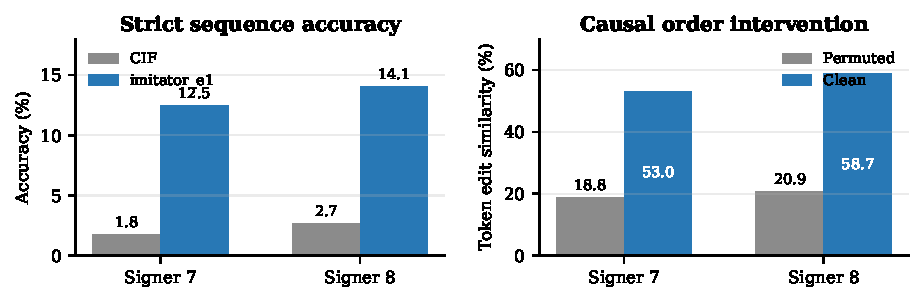
\includegraphics[width=\textwidth]{confirmation_results.pdf}
\caption{Confirmatory evidence on unseen signers. Left: strict sequence accuracy
against the historical CIF comparator. Right: edit similarity collapses when
complete sign segments are permuted while targets remain fixed.}
\label{fig:confirmation-results}
\end{figure}

\begin{figure}[t]
\centering
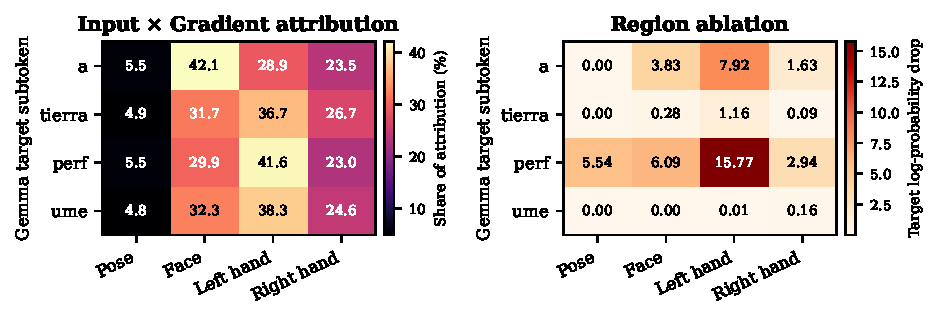
\includegraphics[width=\textwidth]{keypoint_interpretability.pdf}
\caption{Qualitative keypoint interpretation for the target subtokens of an
unseen signer-7 ``A tierra / Perfume'' sequence. Left: normalized
Input$\times$Gradient attribution aggregated into anatomical regions. Right:
decrease in target log-probability when each region is zeroed. Both analyses
identify the left hand as the dominant evidence for the central subtokens; this
single example is descriptive rather than population-level evidence.}
\label{fig:keypoint-interpretability}
\end{figure}

Figure~\ref{fig:keypoint-interpretability} shows that the left hand contributes
28.9--41.6\% of normalized attribution and causes the largest ablation loss for
the central ``a'' and ``perf'' decisions (7.92 and 15.77 log-probability points).
Face keypoints also receive substantial local attribution, whereas their ablation
effect is smaller; this distinction indicates sensitivity without equivalent
causal necessity.  Pose matters mainly for ``perf,'' and the final ``ume'' subtoken
is comparatively insensitive to all four coarse removals.  The agreement between
hand saliency and hand ablation supports a manually grounded decision in this
example, but one selected sequence cannot establish a dataset-wide anatomy claim.

\subsection{Can \Gemma{} repair token errors?}

Table~\ref{tab:gemma-tolerance} answers this question for the current isolated-label
regime.  At zero corruption, \Gemma{} preserves exact content in 95\% of rows and
keeps chrF near 100.  At every tested nonzero rate, exact accuracy is already zero
before correction and remains zero afterward.  chrF decreases rather than improves.
Thus, no nonzero error tolerance is demonstrated: there is no tested nonzero
corruption level at which the language stage recovers exact content.  Because the
short sequences quantize every nonzero nominal rate to at least one substitution,
this experiment does not locate a continuous threshold between 0 and 0.10.

\begin{table}[t]
\centering\small
\caption{\Gemma{} 3n E2B correction audit on 120 isolated-label rows per
condition.  chrF is on a 0--100 scale.  On these short sequences, every nonzero
nominal rate produces at least one substitution.}
\label{tab:gemma-tolerance}
\begin{tabular}{rrrrrr}
\toprule
Substitution rate & Exact before & Exact after & chrF before & chrF after & $\Delta$chrF \\
\midrule
0.00 & 1.000 & 0.950 & 100.00 & 99.16 & -0.84 \\
0.10 & 0.000 & 0.000 & 36.67 & 34.58 & -2.10 \\
0.20 & 0.000 & 0.000 & 36.67 & 34.58 & -2.10 \\
0.30 & 0.000 & 0.000 & 36.67 & 34.58 & -2.10 \\
0.40 & 0.000 & 0.000 & 34.29 & 32.35 & -1.94 \\
0.50 & 0.000 & 0.000 & 23.30 & 21.85 & -1.45 \\
\bottomrule
\end{tabular}
\end{table}

This is not evidence that language models cannot correct sign transcription in
general.  A substitution such as ``photo'' $\rightarrow$ ``green'' in an isolated
label is compatible with no surrounding syntax or semantics that identifies the
original word.  The appropriate next experiment is therefore not another prompt
sweep on LSA64, but a pre-registered sentence corpus in which controlled token
errors leave genuine contextual redundancy.

\section{Discussion}

The main result is an interface result.  Predicting tokenizer IDs turns the original
embedding-imitation idea into an explicit communication channel between the visual
encoder and the LLM.  It also separates two sources of success: \system{} must first
place the correct IDs on that channel; only then can \Gemma{} contribute language
knowledge.  Fluency from the downstream model cannot conceal an incorrect visual
sequence because upstream exact and edit metrics are reported independently.

The current evidence does not yet support the strongest product story---that
\Gemma{} repairs imperfect sign transcription.  It supports the prerequisite:
sign streams from held-out signers can be mapped directly into ordered, valid
\Gemma{} IDs with
substantially higher sequence accuracy than the initial decoder.  The negative
corruption audit explains why correction is absent here and produces a concrete
data requirement for the next stage: natural multiword sentences, multiple
plausible contexts, and enough redundancy that a corrupted token is inferable.

Discrete IDs trade flexibility for auditability.  Unlike continuous prompts, they
do not communicate a calibrated posterior over alternative tokens.  Future work
should compare top-$k$ or posterior-weighted interfaces, as explored in speech
prompting \citep{deng2025wav2prompt,ma2025legoslm}, while retaining a separately
scored visual transcript.  Such uncertainty may give the LLM useful alternatives
without returning to unconstrained embedding imitation.

\section{Limitations and Scope}

LSA64 contains 64 isolated signs \citep{ronchetti2016lsa64}.  Our examples
concatenate two to eight clips, but remain synthetic: they lack coarticulation
and natural sentence order.  The 64-sign inventory limits evaluation to a fixed
vocabulary; these results do not establish lexical coverage for natural
sign-language communication or open-vocabulary translation.  The 121-row output
layer covers only Gemma IDs observed for this task.  Spanish lexical annotations
do not model LSA grammar.  Skeleton inputs omit visual appearance and depend on
pose-estimation quality \citep{harrouch2026manual,nam2026liftsign}.

All reported model results use a single training seed (23), so between-seed
variance and robustness across independent training runs are unknown.  The
sample-level bootstrap intervals quantify uncertainty across evaluated examples,
not variability across training runs, and do not replace signer-level replication.
Only two outer signers are prospectively confirmatory.  \ImitatorEOne{} and the H2
threshold were developed on folds 4--6.
The tokenizer restriction is efficient for a closed label set but must be expanded
and revalidated for sentence data.  Finally, the correction audit tests one model
and a fixed prompt; its defensible conclusion is limited to the tested setup and
rates, although the absence of contextual information is a structural limitation
of the present data.

\section{Conclusion}

\system{} keeps the original goal of learning a lightweight bridge from sign motion
to a pretrained language model, but replaces approximate embedding imitation with
exact token-ID prediction.  This change makes the bridge directly decodable,
measurable, and compatible with an unchanged \Gemma{} text interface.  In the
seed-23 evaluation, signer-held-out tests of synthetic two-to-eight-sign LSA64
streams show improved ordered token transcription.  The correction audit covers
isolated labels at the tested substitution rates and finds no recovery at nonzero
rates; sentence-level correction remains untested.

\section*{Reproducibility and Ethics}

The confirmation configuration, metrics, perturbation seeds, and decision rules
were committed before observing \ImitatorEOne{} outer results for signers 7--8.
The source code and experiment configurations are available at
\url{https://github.com/nakato156/Imitator-E1}. The dataset and trained
checkpoints are not redistributed with that repository; access to LSA64 remains
subject to its own terms. LSA64's source describes ten non-expert subjects wearing
colored gloves \citep{ronchetti2016lsa64}. Public documentation inspected for this
draft does not provide sufficient demographic or consent detail for broader fairness
claims. Although keypoints reduce direct appearance exposure, motion traces remain
biometric data and should not be treated as anonymous by default.



\begin{credits}
\subsubsection{Acknowledgements}
The authors acknowledge the Universidad Peruana de Ciencias Aplicadas for
supporting this research.

\subsubsection{Disclosure of Interests}
The authors have no competing interests to declare that are relevant to the
content of this article.
\end{credits}

\bibliographystyle{splncs04}
\bibliography{../../shared/references}

\end{document}
